%!TEX output_directory = temp
\documentclass[letterpaper, 12pt]{amsart}
	%%%%%%%%%%%%%%%%%%%%%%%%%%%%%%%%%%%%%%%%%%%%%%%%%%%%%%%%%%%%%%%%%%%%%%%%%%%%%%
	%%%%%%%%%%%%%%%%%%%%%%%%%%%% boilerplate packages %%%%%%%%%%%%%%%%%%%%%%%%%%%%
		\usepackage[margin=1.5in]{geometry}
		\usepackage{amsmath,amssymb,amsthm}
		\usepackage{marvosym}
		\usepackage[mathscr]{euscript}
		\usepackage{enumerate}
		\usepackage{graphicx}
		\usepackage{mathrsfs}
		\usepackage{color}
		\usepackage{hyperref}
		\usepackage{verbatim}
		\usepackage{stmaryrd}
		\usepackage{subfigure}

	%%%%%%%%%%%%%%%%%%%%%%%%%%%%%%%%%%%%%%%%%%%%%%%%%%%%%%%%%%%%%%%%%%%%%%%%%%%%%%
	%%%%%%%%%%%%%%%%%%%%%%%%%%%%% rename the abstract %%%%%%%%%%%%%%%%%%%%%%%%%%%%
		% \renewcommand{\abstractname}{Introduction}

	%%%%%%%%%%%%%%%%%%%%%%%%%%%%%%%%%%%%%%%%%%%%%%%%%%%%%%%%%%%%%%%%%%%%%%%%%%%%%%
	%%%%%%%%%%%%%%%%%%%%%%%%%%%%%%%%%%%%% sets %%%%%%%%%%%%%%%%%%%%%%%%%%%%%%%%%%%
		\DeclareMathOperator{\N}{\mathbb{N}}				% natural numbers
		\DeclareMathOperator{\Z}{\mathbb{Z}}				% integers
		\DeclareMathOperator{\Zp}{\mathbb{Z}^{+}}			% positive integers
		\DeclareMathOperator{\Q}{\mathbb{Q}}				% rationals
		\DeclareMathOperator{\Qc}{\mathbb{Q}^{c}}			% irrationals
		\DeclareMathOperator{\R}{\mathbb{R}}				% reals
		\DeclareMathOperator{\F}{\mathbb{F}}				% a field
		\DeclareMathOperator{\C}{\mathbb{C}}				% complex numbers
		\DeclareMathOperator{\Cnon}{\mathbb{C}^{\times}}	% nonzero complex numbers
		\DeclareMathOperator{\Pcal}{\mathcal{P}}			% powerset, or set of polynomials
		\DeclareMathOperator{\Ell}{\mathscr{L}}				% set of linear maps, or linear operator

	%%%%%%%%%%%%%%%%%%%%%%%%%%%%%%%%%%%%%%%%%%%%%%%%%%%%%%%%%%%%%%%%%%%%%%%%%%%%%%
	%%%%%%%%%%%%%%%%%%%%%%%%%%%%%% use pretty letters %%%%%%%%%%%%%%%%%%%%%%%%%%%%
		\DeclareMathOperator{\ep}{\varepsilon}				% epsilons
		\DeclareMathOperator{\ph}{\varphi}					% phis

	%%%%%%%%%%%%%%%%%%%%%%%%%%%%%%%%%%%%%%%%%%%%%%%%%%%%%%%%%%%%%%%%%%%%%%%%%%%%%%
	%%%%%%%%%%%%%%%%%%%%%%%%%%%%%%%%%%% algebra %%%%%%%%%%%%%%%%%%%%%%%%%%%%%%%%%%
		\renewcommand{\null}{\text{null }}					% null space
		\DeclareMathOperator{\range}{\text{range }}			% range
		\newcommand{\bmat}[1]{{\mathbf{#1}}}				% bold matrix
		\newcommand{\bvec}[1]{{\vec{\mathbf{#1}}}}			% bold vector
		\DeclareMathOperator{\ind}{\perp\!\!\!\perp}		% perpendicular, orthogonal
		\DeclareMathOperator{\ord}{\text{ord}}				% order of a structure
		\DeclareMathOperator{\Log}{Log}						% logarithm
		\DeclareMathOperator{\Span}{Span}					% span
		\newcommand{\pid}[1]{\langle #1 \rangle}			% bracket notation, used for 
															% ideals or inner products
		\newcommand{\norm}[1]{\mid \!\!#1 \!\!\mid}			%\norm{x} gives |x|

		% fatdot notation
		\makeatletter
			\newcommand*\fatdot{\mathpalette\fatdot@{.5}}
			\newcommand*\fatdot@[2]{\mathbin{\vcenter{\hbox{\scalebox{#2}{$\m@th#1\bullet$}}}}}
		\makeatother

	%%%%%%%%%%%%%%%%%%%%%%%%%%%%%%%%%%%%%%%%%%%%%%%%%%%%%%%%%%%%%%%%%%%%%%%%%%%%%%
	%%%%%%%%%%%%%%%%%%%%%%%%%%% probability & statistics %%%%%%%%%%%%%%%%%%%%%%%%%
		\renewcommand{\Pr}{\mathbb{P}}						% probability
		\DeclareMathOperator{\E}{\mathbb{E}}				% expectation
		\DeclareMathOperator{\var}{\rm Var}					% variance
		\DeclareMathOperator{\sd}{\rm SD}					% standard deviation
		\DeclareMathOperator{\cov}{\rm Cov}					% covariance
		\DeclareMathOperator{\SE}{\rm SE}					% standard error
		\DeclareMathOperator{\ssreg}{{\rm SS}_{{\rm Reg}}}	% sum of squared regression
		\DeclareMathOperator{\ssr}{{\rm SS}_{{\rm Res}}}	% sum of squared residuals
		\DeclareMathOperator{\sst}{{\rm SS}_{{\rm Tot}}}	% total sum of squares

	%%%%%%%%%%%%%%%%%%%%%%%%%%%%%%%%%%%%%%%%%%%%%%%%%%%%%%%%%%%%%%%%%%%%%%%%%%%%%%
	%%%%%%%%%%%%%%%%%%%%%%%%%%%%%%% number theory %%%%%%%%%%%%%%%%%%%%%%%%%%%%%%%%
		\renewcommand{\mod}[1]{\ (\mathrm{mod}\ #1)}		% congruences

	%%%%%%%%%%%%%%%%%%%%%%%%%%%%%%%%%%%%%%%%%%%%%%%%%%%%%%%%%%%%%%%%%%%%%%%%%%%%%%
	%%%%%%%%%%%%%%%%%%%%%%%%%%%% theorem environments %%%%%%%%%%%%%%%%%%%%%%%%%%%%
		% Some theorem-like environments, all numbered together starting at 1
		% in each section.

		\newtheorem{thm}{Theorem}[section]					% The default \theoremstyle is 
		\newtheorem{defn}[thm]{Definition}					% bold headings and italic body text.
		\newtheorem{prop}[thm]{Proposition}
		\newtheorem{claim}[thm]{Claim}
		\newtheorem{cor}[thm]{Corollary}
		\newtheorem{lemma}[thm]{Lemma}

		\theoremstyle{definition}  							% Bold headings and Roman body text.
		\newtheorem{example}[thm]{Example}
		\newtheorem{examples}[thm]{Examples}
		\newtheorem{exercise}[thm]{Exercise}
		\newtheorem{note}[thm]{Note}
		\newtheorem{remark}[thm]{Remark}
		\newtheorem{remarks}[thm]{Remarks}
		\newtheorem{discussion}[thm]{Discussion}

		\newcommand{\dfn}{\textbf} 							% Make defined words bold.
		\newcommand{\mdfn}[1]{\dfn{\mathversion{bold}#1}} 	% Even make math symbols bold

	%%%%%%%%%%%%%%%%%%%%%%%%%%%%%%%%%%%%%%%%%%%%%%%%%%%%%%%%%%%%%%%%%%%%%%%%%%%%%%
	%%%%%%%%%%%%%%%%%%%%%%%%%%%%%%% complex numbers %%%%%%%%%%%%%%%%%%%%%%%%%%%%%%
		\DeclareMathOperator{\Arg}{Arg}						% argument of z \in \C
		\DeclareMathOperator{\re}{Re}						% real component
		\DeclareMathOperator{\im}{Im}						% imaginary component

	%%%%%%%%%%%%%%%%%%%%%%%%%%%%%%%%%%%%%%%%%%%%%%%%%%%%%%%%%%%%%%%%%%%%%%%%%%%%%%
	%%%%%%%%%%%%%%%%%%%%%%%%%%%%%%% various symbols %%%%%%%%%%%%%%%%%%%%%%%%%%%%%%
		\newcommand{\iso}{\cong}						% isometric/congruent
		\newcommand{\ra}{\rightarrow}                   % right arrow
		\newcommand{\Ra}{\Rightarrow}                   % right implies
		\newcommand{\lra}{\longrightarrow}              % long right arrow
		\newcommand{\la}{\leftarrow}                    % left arrow
		\newcommand{\La}{\Leftarrow}                    % left implies
		\newcommand{\lla}{\longleftarrow}               % long left arrow
		\newcommand{\eqra}{\llra{\sim}}                 % equivalence/isomorphism
		\newcommand{\blank}{\underbar{\ \ }}          	% An underscore, as in (__)xV
		% \newcommand{\blank}{-}                          % A hyphen, as in (-)xV
		\newcommand{\Id}{Id}                            % The identity functor
		\newcommand{\und}{\underline}
		\newcommand{\del}{\nabla}						% gradient vector

		\raggedbottom	
\begin{document}
	\title{Homework 5  -- Math 397 \\ \today}
	\author{Alex Thies \\ \href{mailto:athies@uoregon.edu}{\lowercase{athies$@$uoregon.edu}}}

	\maketitle

	\section*{Exercise 1}
		\subsection*{Part (a)}
		Use Sage to plot the polar-coordinate equaton $r = \tfrac{1}{3-\cos\theta}$. 
		Then plot the similar $r = \tfrac{1}{3-\lambda\cos\theta}$ equations for various values of $\lambda$ stretching from 1 to 7. 
		What happens to the graph? 
		What value of $\lambda$ produces an ellipse that stretches all the way out to $x = 100$?

		\begin{proof}[Solution]
		Here are some of the more interesting outputs from playing around with this in Sage.
		Figures \ref{lambda_1} and \ref{lambda_2} show the ellipses that we expect.
		Notice that Figure \ref{lambda_299} shows that the ellipse stretches to $x=100$ when $\lambda = 2.99$, i.e., when $\lambda$ is quite close to 3.
		We also have the interesting parabolas and hyperbolas in Figures \ref{lambda_3}, \ref{lambda_35} and \ref{lambda_4}.
		Unfortunately, for these three graphs, I was unable to determine how to turn off the oblique asymptotes from appearing as they do.

		\begin{figure*}[b]
			\centering
			\begin{minipage}[b]{.4\textwidth}
				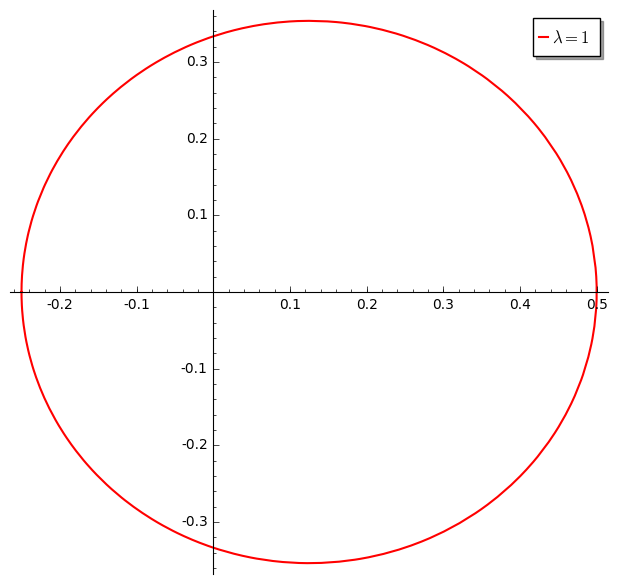
\includegraphics[scale=0.38]{images/lambda1.png}
				\caption{$r(\theta)$ when $\lambda = 1$.}
				\label{lambda_1}
			\end{minipage}
			\qquad
			\begin{minipage}[b]{.4\textwidth}
				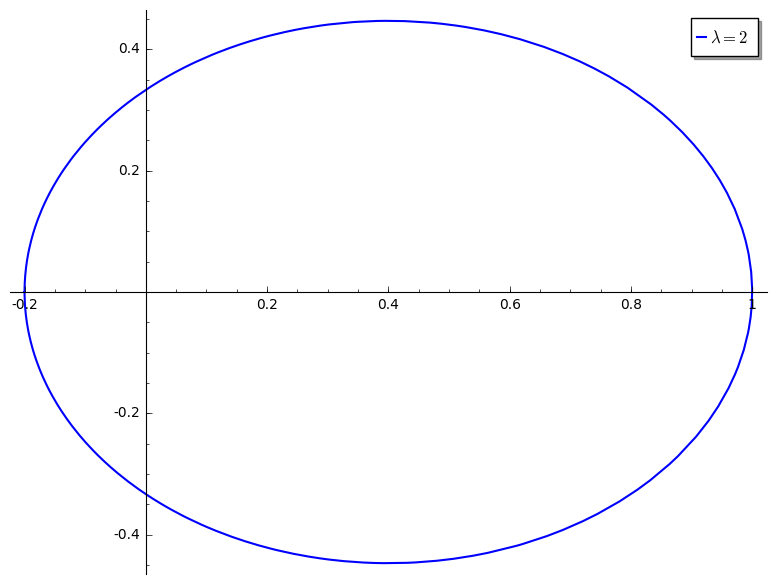
\includegraphics[scale=0.38]{images/lambda2.png}
				\caption{$r(\theta)$ when $\lambda = 2$.}
				\label{lambda_2}
			\end{minipage}
		\end{figure*}
		\end{proof}
		% subsection part_a (end)

		\subsection*{Part (b)}
		Now do the algebra that explains what is happening in part (a). 
		Start with $r = \tfrac{1}{3-\lambda\cos\theta}$ and rewrite that as $$1 = r(3-\lambda\cos\theta).$$
		Change to Cartesian coordinates using $r = \sqrt{x^2 + y^2}$ and $r \cos\theta = x$. 
		Do some algebra, get rid of square roots, and rearrange until you get a quadric equation. 
		What values of $\lambda$ give the different types of conics? 
		The review of quadric equations below might be helpful.\footnote{Omitted.}

		\begin{proof}[Solution]
		We compute the following,
			\begin{align*}
				r &= \frac{1}{3-\lambda\cos\theta}, \\
				1 &= r(3-\lambda\cos\theta), \\
				&= 3\sqrt{x^2+y^2} - \lambda x, \\
				1 + \lambda x &= 3\sqrt{x^2+y^2}, \\
				1 + 2\lambda x + \lambda^2x^2 &= 9x^2 + 9y^2, \\
				0 &= \left( 9 - \lambda^2 \right)x^{2} + 9y^2 - 2\lambda x - 1.
			\end{align*}
		Hence, we have a quadric equation where $A = 9 - \lambda^2$, $B = 9$, $C = -2\lambda$, and $D = -1$.
		Next, we will complete the square.

		\begin{figure*}[b]
			\centering
			\begin{minipage}[b]{.4\textwidth}
				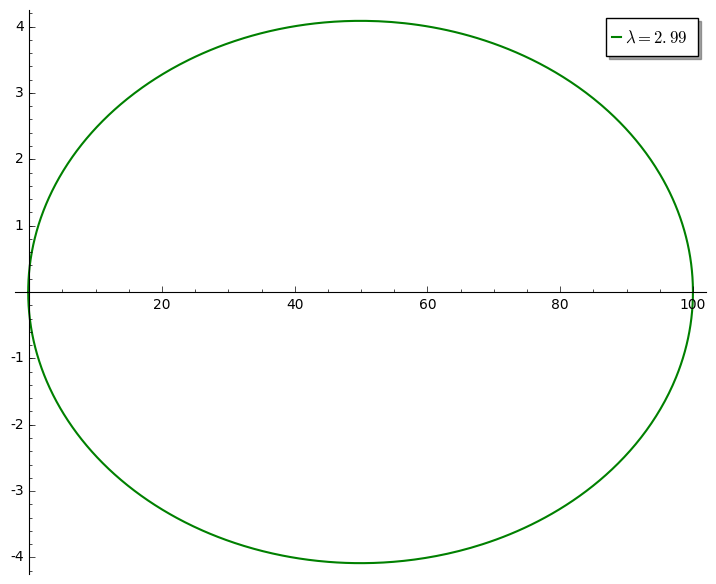
\includegraphics[scale=0.35]{images/lambda299.png}
				\caption{$r(\theta)$ when $\lambda = 2.99$.}
				\label{lambda_299}
			\end{minipage}
			\qquad
			\begin{minipage}[b]{.4\textwidth}
				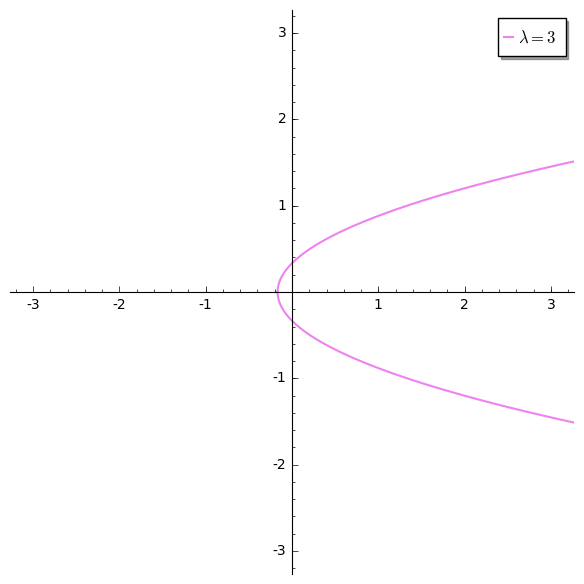
\includegraphics[scale=0.35]{images/lambda3.png}
				\caption{$r(\theta)$ when $\lambda = 3$.}
				\label{lambda_3}
			\end{minipage}
		\end{figure*}

			\begin{align*}
				0 &= \left( 9 - \lambda^2 \right)x^{2} + 9y^2 - 2\lambda x - 1, \\
				&= \left( 9 - \lambda^2 \right)x^{2} - 2\lambda x + 9y^2  - 1, \\
				&= \left( 9 - \lambda^2 \right)\left(x^2 - \tfrac{2\lambda}{9 - \lambda^2}x \right) + 9y^2 - 1, \\
				&= \left( 9 - \lambda^2 \right)\left(x - \tfrac{2\lambda}{2\left(9 - \lambda^2\right)}x \right)^{2} + 9y^2 - 1 - \tfrac{4\lambda^2}{4(9 - \lambda^2)^2}, \\
				&= \left( 9 - \lambda^2 \right)u^{2} + 9y^2 - \tfrac{(9 - \lambda^2)^2 - \lambda^2}{(9 - \lambda^2)^2}, \\
				&= \left( 9 - \lambda^2 \right)u^{2} + 9y^2 - \tfrac{\lambda^2 - 18\lambda + 81 - \lambda^2}{\lambda^4 - 18\lambda^2 + 81}, \\
				&= \left( 9 - \lambda^2 \right)u^{2} + 9y^2 - \tfrac{9(9 - 2\lambda)}{(9 - \lambda^2)^2}, \\
				&= \left( 9 - \lambda^2 \right)u^{2} + 9y^2 + E, \\
				& \text{Where $u = x - \tfrac{2\lambda}{2\left(9 - \lambda^2\right)}x$, and $E = - \tfrac{9(9 - 2\lambda)}{(9 - \lambda^2)^2}$.}
			\end{align*}

		\begin{figure*}[b]
			\centering
			\begin{minipage}[b]{.4\textwidth}
				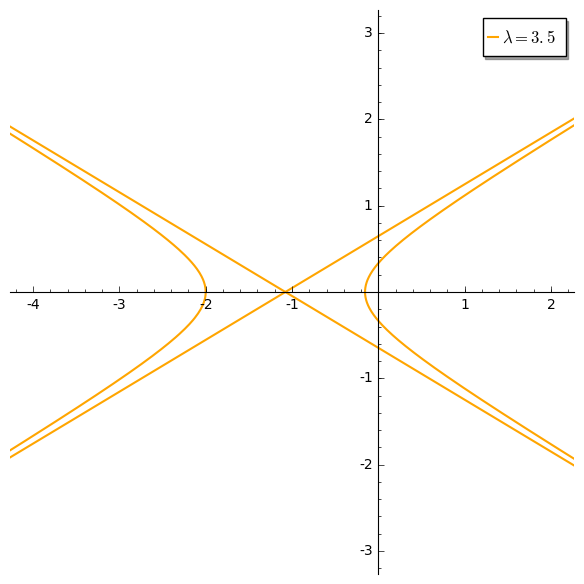
\includegraphics[scale=0.38]{images/lambda35.png}
				\caption{$r(\theta)$ when $\lambda = 3.5$.}
				\label{lambda_35}
			\end{minipage}
			\qquad
			\begin{minipage}[b]{.4\textwidth}
				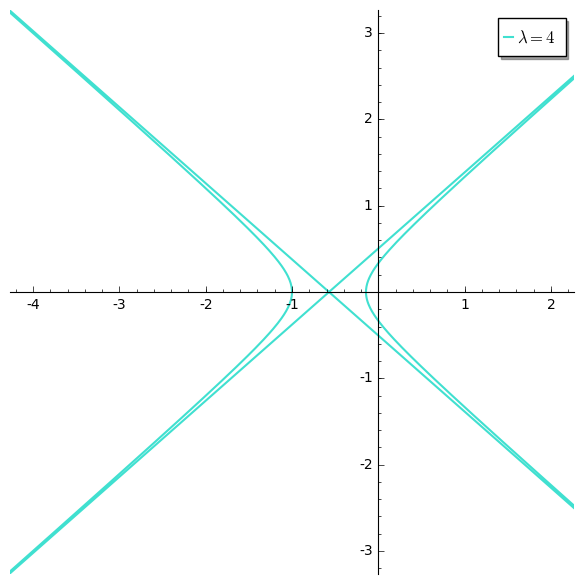
\includegraphics[scale=0.38]{images/lambda4.png}
				\caption{$r(\theta)$ when $\lambda = 4$.}
				\label{lambda_4}
			\end{minipage}
		\end{figure*}
		\end{proof}
		% subsection part_b (end)

		\subsection*{Part (c)}
		Show that an ellipse $Ax^2 + By^2 = C$ has eccentricity $\sqrt{1 - \tfrac{B}{A}}$ if $B \leq A$ (or alternatively, $\sqrt{1 - \tfrac{A}{B}}$ when $A \leq B$).

		\begin{proof}[Solution]
		Recall that for an ellipse 
			\begin{equation}\label{ellipse}
				\frac{x^2}{a^2} + \frac{y^2}{b^2} = 1
			\end{equation}
		the eccentricity $e$ is defined as 
			\begin{equation}\label{eccentricity}
				e = \sqrt{1 - \left(\tfrac{b}{a}\right)^2}
			\end{equation}
		Notice that for $Ax^2 + By^2 = C$ we have $a = \sqrt{C/A}$ and $b = \sqrt{C/B}$.
		Assume $B \leq A$.
		Then we have 
			\begin{align*}
				e &= \sqrt{1 - \left(\tfrac{a}{b}\right)^2}, \\
				&= \sqrt{1 - \left( \frac{\sqrt{C/A}}{\sqrt{C/B}} \right)^2}, \\
				&= \sqrt{1 - \frac{C/A}{C/B}}, \\
				&= \sqrt{1 - \frac{1/A}{1/B}}, \\
				&= \sqrt{1 - \frac{A^{-1}}{B^{-1}}}, \\
				&= \sqrt{1 - \frac{B}{A}}.
			\end{align*}
		\end{proof}
		% subsection part_c (end)

		\subsection*{Part (d)}
		Using your work in (b), derive a formula for the eccentricity of the ellipse $r = \tfrac{1}{3-\lambda\cos\theta}$ in terms of $\lambda$.

		\begin{proof}[Solution]
		Recall we have $A = 9 - \lambda^2$ and $B = 9$, if we assume $B \leq A$, we arrive at a contradiction that $\lambda^2 \leq 0$, so assume $A \leq B$, i.e., $\lambda^2 \geq 0$.
		Then by part (c) we have $$e = \sqrt{1 - \frac{9 - \lambda^2}{9}}.$$
			
		But I also did it the hard way before realizing that I didn't have to...
		This requires us to change $\left( 9 - \lambda^2 \right)u^{2} + 9y^2 + E$ into the form of (\ref{ellipse}).
		We compute the following,
			\begin{align*}
				0 &= \left( 9 - \lambda^2 \right)u^{2} + 9y^2 - \tfrac{9(9 - 2\lambda)}{(9 - \lambda^2)^2}, \\
				\tfrac{9(9 - 2\lambda)}{(9 - \lambda^2)^2} &= \left( 9 - \lambda^2 \right)u^{2} + 9y^2, \\
				\frac{\tfrac{9(9 - 2\lambda)}{(9 - \lambda^2)^2}}{\tfrac{9(9 - 2\lambda)}{(9 - \lambda^2)^2}} &= \frac{\left( 9 - \lambda^2 \right)u^{2}}{\tfrac{9(9 - 2\lambda)}{(9 - \lambda^2)^2}} + \frac{9y^2}{\tfrac{9(9 - 2\lambda)}{(9 - \lambda^2)^2}}, \\
				1 &= u^{2} \left( (9 - \lambda^2) \frac{(9 - \lambda^2)^2}{9(9 - 2\lambda)} \right) + y^{2}\left( 9 \frac{(9 - \lambda^2)^2}{9(9 - 2\lambda)} \right), \\
				1 &= u^{2} \left( \frac{(9 - \lambda^2)^3}{9(9 - 2\lambda)} \right) + y^{2}\left( \frac{(9 - \lambda^2)^2}{(9 - 2\lambda)} \right), \\
				1 &= \frac{u^{2}}{\tfrac{{9(9 - 2\lambda)}}{{(9 - \lambda^2)^3}}} + \frac{y^{2}}{\tfrac{{(9 - 2\lambda)}}{{(9 - \lambda^2)^2}}}.
			\end{align*}
		Hence, we have $$a = \sqrt{\tfrac{{9(9 - 2\lambda)}}{{(9 - \lambda^2)^3}}} \hspace{2.5mm} \text{and} \hspace{2.5mm} b = \sqrt{\tfrac{{(9 - 2\lambda)}}{{(9 - \lambda^2)^2}}}.$$
		We can proceed to formulate $e$.
			\begin{align*}
				e &= \sqrt{1 - \left(\frac{b}{a}\right)^2}, \\
				&= \sqrt{1 - \left( \frac{\sqrt{\tfrac{{(9 - 2\lambda)}}{{(9 - \lambda^2)^2}}}}{\sqrt{\tfrac{{9(9 - 2\lambda)}}{{(9 - \lambda^2)^3}}}} \right)^2}, \\
				&= \sqrt{1 - \frac{\tfrac{{(9 - 2\lambda)}}{{(9 - \lambda^2)^2}}}{\tfrac{{9(9 - 2\lambda)}}{{(9 - \lambda^2)^3}}} }, \\
				&= \sqrt{1 - \frac{{(9 - 2\lambda)}}{{(9 - \lambda^2)^2}} \cdot \frac{{(9 - \lambda^2)^3}}{{9(9 - 2\lambda)}}}, \\
				&= \sqrt{1 - \frac{9 - \lambda^2}{9}}.
			\end{align*}
		However we get here, it becomes clear why $\lambda = 3$ and $\lambda > 3$ from part (a) have such interesting behavior.			
		\end{proof}
		% subsection part_d (end)
		\newpage

		\subsection*{Part (e)}
		Thinking about all the above parts, fill in the blanks for the following ``morals'' (statements that are not technically true but nevertheless have some interesting content to them):
		$$ \text{an ellipse with eccentricity $e = 1$ is really a \, $\blank\blank\blank\blank\blank\blank\blank\blank\blank\blank\blank\blank\blank\blank\blank$}$$
		\vspace{2mm}
		$$ \text{an ellipse with eccentricity $e > 1$ is really a \, $\blank\blank\blank\blank\blank\blank\blank\blank\blank\blank\blank\blank\blank\blank\blank$}$$
		% subsection part_e (end)
	% section exercise_1 (end)

	\section*{Exercise 2}
	The Runge-Kutta order 4 method is, for the most part, extremely reliable. 
	This problem will show you a place where you need to be careful, though.
		\subsection*{Part (a)}
		Solve the separable differential equation $y' = \tfrac{-x}{y}, \, y(0) = 2$ and show that the solution is $y(x) = \sqrt{4 - x^2}$. 
		What will the graph look like?

		\begin{proof}[Solution]
		We compute the following,
			\begin{align*}
			\frac{dy}{dx} &= \frac{-x}{y}, \\
			y \, dy &= -x \, dx, \\
			\int y \, dy &= - \int x \, dx, \\
			\frac{y^2}{2} &= \frac{-x^2}{2} + C, \\
			y^2 &= -x^2 + C, \\
			y &= \sqrt{C - x^2}.
			\end{align*}
			Now, we apply the initial condition.
			\begin{align*}
			y(0) = 2 &= \sqrt{C - 0^2}, \\
			2 &= \sqrt{C}, \\
			C &= 4.
			\end{align*}
			\pagebreak

			Hence, we have the particular solution $y(x) = \sqrt{4 - x^2}$.
			Notice that the domain of $y(x)$ is $[-2,2]$, and that the maximum value of $y(x)$ is $y(0)=2$.
			Hence, this solution will look like an upside-down parabola with roots at $x=\pm2$ and vertex at $(0,2)$.
			See Figure \ref{partSoln1} for a picture.

			\begin{figure}[b]
				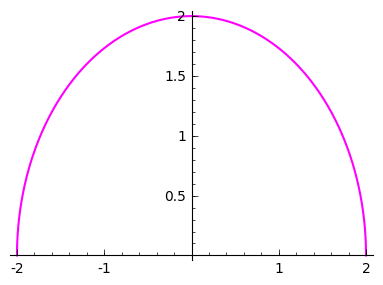
\includegraphics[width=0.45\textwidth]{images/partSoln1.png}
				\caption{$y(x) = \sqrt{4 - x^2}$}
				\label{partSoln1}
			\end{figure}
		\end{proof}
		% subsection part_a (end)

		\subsection*{Part (b)}
		Now try the Sage commands
		$$\verb|P = desolve_rk4(-x,y,y,ivar=x,ics=[0,2],endpoints=10,step=0.5)|$$
		$$\verb|points(P)|$$
		You will see something kind of crazy, not looking very much like what you expected. 
		Try changing the step size to 0.1; it is even crazier!

		Focus on the region where you expect the function to be defined, and blow up the graph accordingly. 
		Include the graph as your solution to this part. 
		You might have to use the ``aspect ratio'' feature (see previous homeworks) to make the graph look right.

		\begin{proof}[Solution]
			Using Sage we create the graph found in Figure \ref{SlopeFieldSoln}.
		\end{proof}
		% subsection part_b (end)

		\subsection*{Part (c)}
		Numerical approximations to first-order differential equations use the slopes of the tangent lines to advance the solution from one point to the next. 
		Keeping that in mind, what do you think is going wrong with this particular differential equation that is confusing Sage? 
		Consider plotting the points on a slope field.

		\begin{proof}[Solution]
		Based on changing the step-size in Figure \ref{SlopeFieldSoln}, we can see that Sage doesn't take into consideration tangent lines that pull a solution out of the domain of the particular solution.
		In this case, we have a particular solution $y(x)$ is domain $[-2,2]$.
		Looking at Figure \ref{SlopeFieldSoln}, consider either of the red or blue dots that is at the very end of $y(x)$ on the right-hand side.
		Picture the tangent lines to $y(x)$ at each of those points.
		Notice that these tangent lines wander outside of the domain of $y(x)$, and, as I like to say, go bananas.
		This is interesting to look at after making absurdly small step-sizes, as in Figure \ref{bananas}.
		We can see that by `buying more accuracy' within our practical domain of $[0,2]$, we incur `bananas'-like behavior on the interval $(2,\infty)$.
			\begin{figure}[h]
				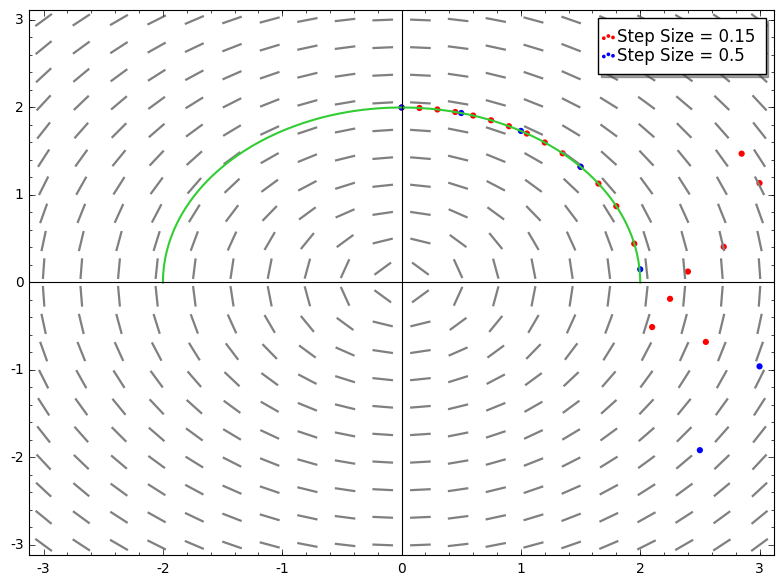
\includegraphics[width=0.7\textwidth]{images/slopeFieldSoln.png}
				\caption{Graph of ODE Solutions}
				\label{SlopeFieldSoln}
			\end{figure}
			\begin{figure}[h]
				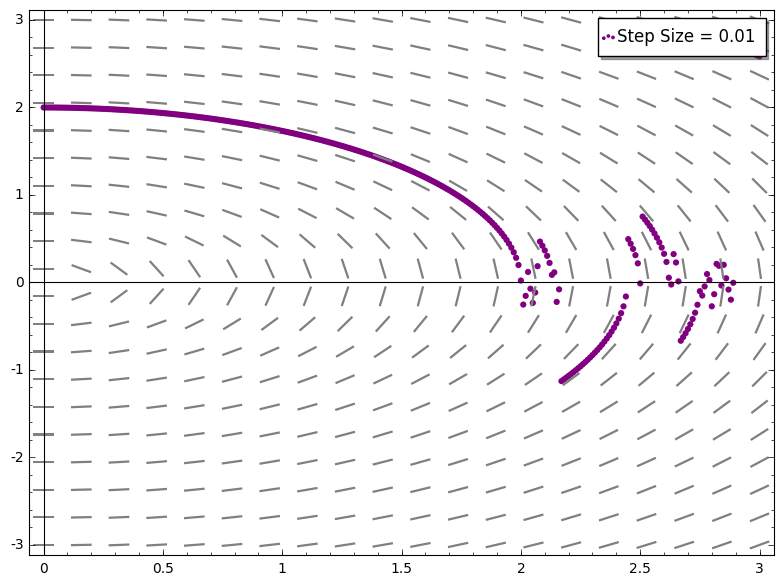
\includegraphics[width=0.7\textwidth]{images/bananas.png}
				\caption{Graph of ODE Solutions with small step-size}
				\label{bananas}
			\end{figure}
		\end{proof}
		% subsection part_c (end)
	% section exercise_2 (end)

	\section*{Exercise 3}
	This problem deals with a pendulum of length $\ell$. 
	Deriving the differential equation for a pendulum is not too difficult.\footnote{Read about it in the Acheson chapter or in the pdf posted with assignment.}
	It is $$\theta'' = -\tfrac{g}{\ell} \cdot \sin\theta,$$ which is nonlinear and hard to solve. 
	You can then use the approximation $\sin(\theta) \approx \theta$ (good for small angles) and change it to $$\theta'' = -\tfrac{g}{\ell} \cdot \theta,$$ which can be solved to find $\theta = A \sin(\omega t) + B \cos(\omega t)$ where $\omega = 􏰃\sqrt{g/\ell}$. 
	In this problem we will explore the differences between our approximate model and the true pendulum. 
	For convenience, let’s just take $\ell = g$ so that $\omega = 1$. 
	The mathematics is the same no matter what the constant $g$ is, so making it 1 doesn’t hurt as far as exploring the main ideas.
	Also, one tends to think of a pendulum as a mass suspended from a string, but in this problem we will consider pendulums that go 360 degrees around. 
	In this case, the pendulum forces the mass to always be a distance $\ell$ from the origin, and so it is better to mentally replace the string with a very light rod as this is a more accurate physical model.

		\subsection*{Part (a)}
		Solve the differential equation $\theta'' = -\theta$ with $\theta(0) = 0.5$ and $\theta'(0) = 0$.

		\begin{proof}[Solution]
		Since we are given $\omega = 1$, this becomes pretty simple.
		For a differential equation of this type, we have the general solution $\theta(t) = A \sin(t) + B \cos(t)$, we also have $\theta'(t) = A \cos(t) - B \sin(t)$.
		Applying the initial conditions to each yields $A = 0$ and $B = 1/2$, thus we have the particular solution $$\theta(t) = \tfrac{1}{2}\cos{t}.$$
		\end{proof}
		% subsection part_a (end)

		\subsection*{Part (b)}
		Set $z = \theta'$ so that for our ``true pendulum'' we get the system of first-order equations $$\theta' = z, \hspace{5mm} z' = -\sin\theta$$
		Use the initial conditions $\theta(0) = 0.5$ and $\theta'(0) = 0$ (so the pendulum is released from a resting position). 
		The solution for our approximate model is $\theta(t) = 0.5 \cos(t)$. 
		Use Sage to compute a numerical solution to the true pendulum, and plot it on the same graph as our approximate solution. 
		Plot a time period of at least $[0, 20]$ so that you can see how the two solutions compare over time.\footnote{Note that you can use “theta” as a variable in Sage as long as you introduce it via the command var('theta').}
		If you do this correctly, you should find that the true solution and our approximate solution are pretty close. Include the graph as your solution to this part.

		\begin{proof}[Solution]
		We have the graph of the ``true pendulum'' against the ``simple pendulum'' in Figure \ref{theta1}.

			\begin{figure}[b]
				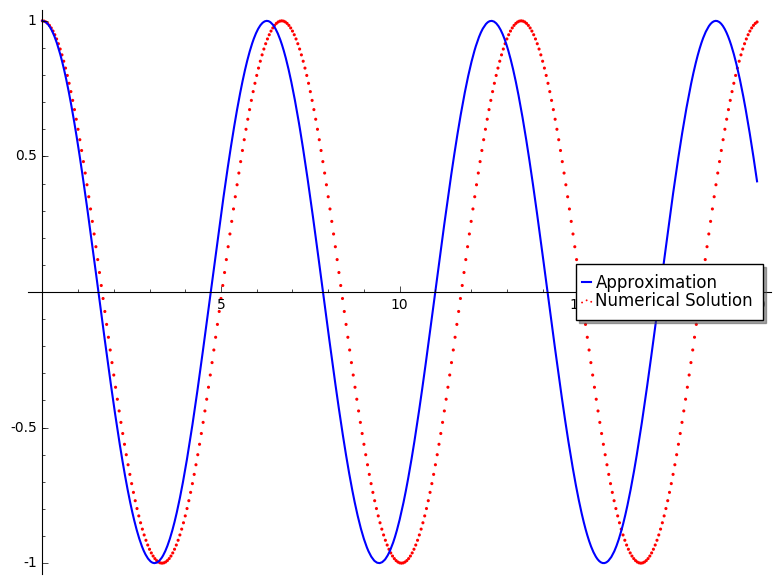
\includegraphics[width=0.75\textwidth]{images/theta1.png}
				\caption{Solutions to the ODE when $\theta(0)=0.5$, and $\theta'(0)=0$}
				\label{theta1}
			\end{figure}
		\end{proof}
		% subsection part_b (end)

		\subsection*{Part (c)}
		Now change the initial condtions to $\theta(0) = 1$ and repeat. 
		Compare the results to $\theta(0) = 2$ and $\theta(0) = 3$. 
		Give a physical interpretation of how the true pendulum's motion when $\theta(0) = 3$ differs from our approximate model.

		\begin{proof}[Solution]
		This portion of the assignment requires some imagination.
		I found myself recalling to memories of me as child playing with the pendulum on a grandfather clock, usually while bored at my grandparents house.
		But even with these memories of how pendulums work in practice, in order to make sense of these graphs I realized we have to make certain assumptions.
		The first assumption is that we can rotate the pendulum so that it is totally 'upside down' and leave it there, undisturbed. 
		This is due to the fact that we are working with models from the point-mass system of mechanics.
		Second, we disregard all forces that could slow down the pendulum as it swings (other than gravity), these include air resistance and friction, however miniscule they may be.
		Now picture the pendulum from a grandfather clock, but removed from the case so that it can make complete rotations without hitting anything.
		Imagine for how long that pendulum would continue to spin once whipped around by a toddler, if the only thing slowing it down was gravity.
		This helps explain these graphs to an extent, but we also need to wrap our minds around the trigonometry working in background.
		The horizontal axis is in terms of time $t$, and the vertical axis is in terms of of the angle $\theta(t)$ in the counterclockwise direction from the equilibrium position.
		For this reason, it makes sense to assume $0 \leq \theta \leq \pi$, therefore initial conditions for $\theta$ greater than $\pi$ will have interesting results.
		Further, consider that when thinking of the practical use of a pendulum, say in a clock, based on our definition above, the ``working range'' for $\theta$ would be $-\pi/2 \leq \theta \leq \pi/2$.
		Finally, note that if we greatly extend the $t$-axis, we see that $\theta(t)$ for the ``true pendulum'' is quasiperiodic, trending towards $0$ as $t$ approaches $\infty$, which is what we'd hope to see.
		\vspace{4mm}

		Observe Figure \ref{theta3} for the graph of the ``true pendulum'' against the ``simple pendulum'' when $\theta_{0} = 3$.
		Since $3$ is close to $\pi$, this initial condition is the case where we drop the pendulum from nearly straight up, the graph indicates that we should see the pendulum bob `hang' for a moment as it reaches the top of each swing.
		Recalling the grandfather clock helps to explain this situation.

			\begin{figure}[b]
				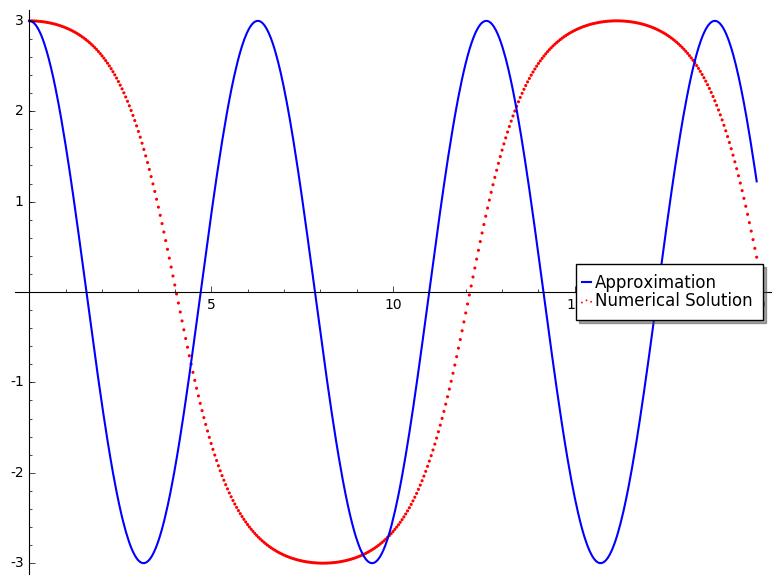
\includegraphics[width=0.65\textwidth]{images/theta3.png}
				\caption{Solutions to the ODE when $\theta(0)=3$, and $\theta'(0)=0$}
				\label{theta3}
			\end{figure}
		\end{proof}
		% subsection part_c (end)

		\subsection*{Part (d)}
		Try the initial condition $\theta(0) = 3.1415$. 
		Then try $\theta(0) = \pi$ (using ``pi'' in Sage). 
		Explain what is happening here.

		\begin{proof}[Solution]
		Observe Figures \ref{theta314} and \ref{thetapi} for the graph of the ``true pendulum'' against the ``simple pendulum'' when $\theta_{0} = 3.1415$ and when $\theta_{0} = \pi$.
		We can see in Figure \ref{theta314} that when the pendulum is dropped from nearly $\pi$, it slowly falls until it sharlpy drops around to the top, but measured in terms of $-\theta$, like we'd expect to see.
		It would continue in this manner for quite awhile, likely due to the lack of damping forces acting on it in our model.
		In the case where $\theta_{0} = \pi$ we see in Figure \ref{thetapi} the case that I alluded to above, where the pendulum is standing straight up.
		\begin{figure}[b]
			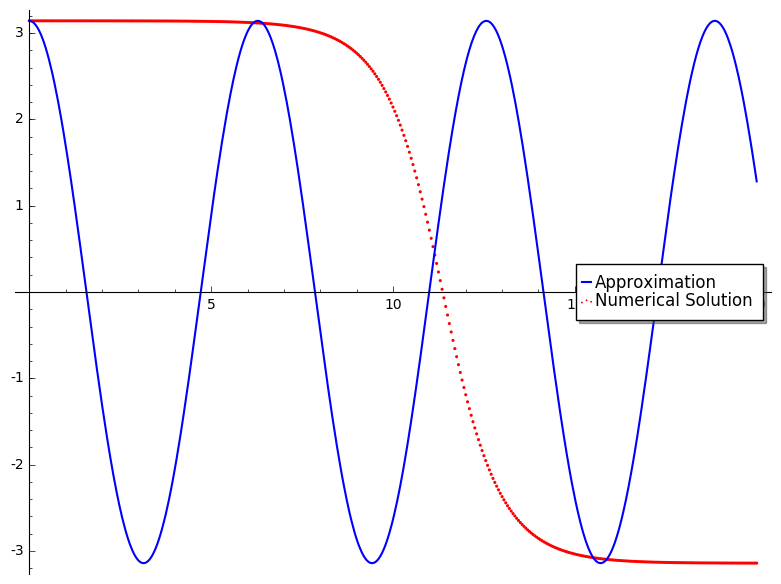
\includegraphics[width=0.65\textwidth]{images/theta314.png}
			\caption{Solutions to the ODE when $\theta(0)=3.1415$, and $\theta'(0)=0$}
			\label{theta314}
		\end{figure}
		\begin{figure}[b]
			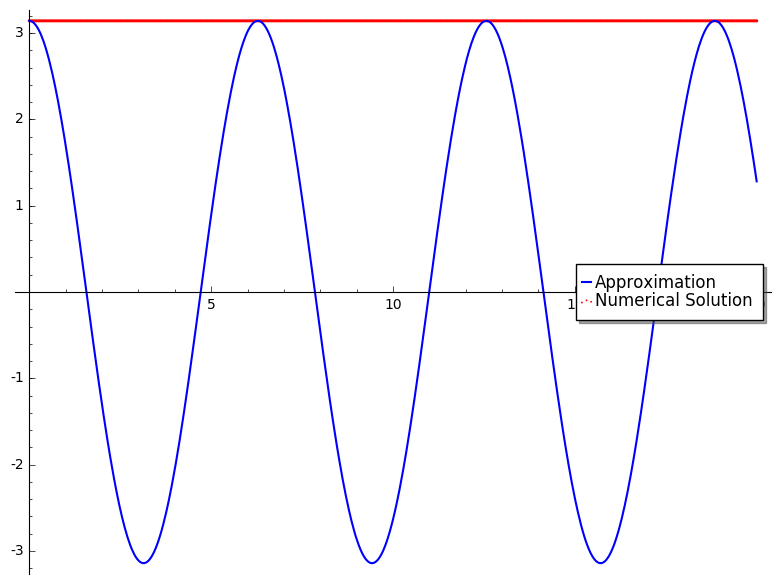
\includegraphics[width=0.65\textwidth]{images/thetapi.png}
			\caption{Solutions to the ODE when $\theta(0)=\pi$, and $\theta'(0)=0$}
			\label{thetapi}
		\end{figure}
		\end{proof}
		% subsection part_d (end)

		\subsection*{Part (e)}
		Set the initial condition as $\theta(0) = 4.5$ and look at the resulting graph. 
		Why is the sine wave shifted vertically up now?

		\begin{proof}[Solution]
		Observe Figure \ref{theta45} for this pretty weird result.
		Recall that we restricted meaningful values of $\theta$ to $[0,\pi]$.
		Therefore, $\theta(0)=4.5$ is the case where we rotate the pendulum more than a half-rotation, dropping it from a place normally reserved for negative values of $\theta$ (this explains the reflection).
		The vertical shift is explained by the fact that when dropping the pendulum from more than a half-rotation, as it swings it not only completes a full $2\pi$ rotation, but it goes beyond $2\pi$, in a part of the circle where we typically measure values of $\theta$ between $0$ and $\pi$.

		\begin{figure}[b]
			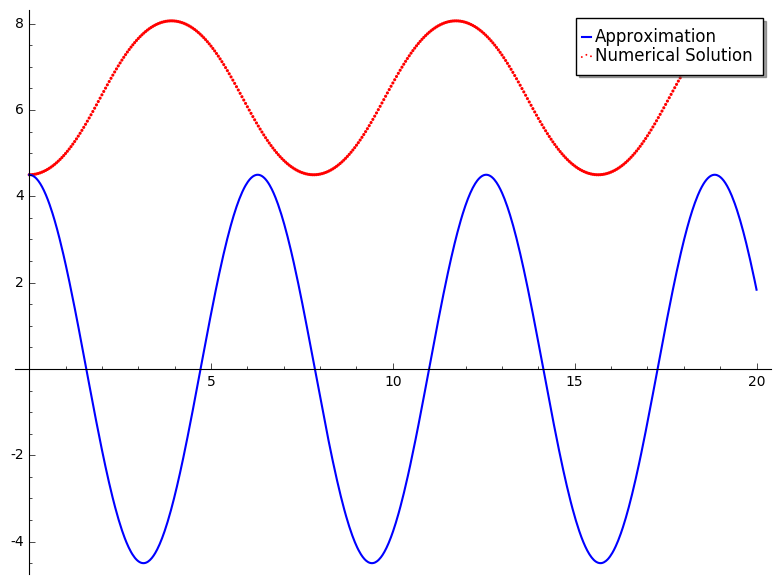
\includegraphics[width=0.65\textwidth]{images/theta45.png}
			\caption{Solutions to the ODE when $\theta(0)=4.5$, and $\theta'(0)=0$}
			\label{theta45}
		\end{figure}
		\end{proof}
		% subsection part_e (end)

		\subsection*{Part (f)}
		Now let’s change the situation, so that the pendulum starts at the bottom $(\theta(0) = 0)$ but we give it an initial velocity $\theta'(0) = 1$. 
		Compute the solution to $\theta'' = -\theta$ for this initial condition, and then plot the numerical model for the true pendulum on the same graph. 
		Use a time interval of at least $[0, 40]$ here.

		\begin{proof}[Solution]
		When $\theta(0)=0$ and $\theta'(0)=1$, we get the particular solution $\theta(t) = \sin{t}$, and generally for $\theta'(0) = \theta'_{0}$, the particular solution is $\theta(t) = \theta'_{0}\sin{t}$. 
		We can see the resulting graph in Figure \ref{fastTheta1}.
		As all of our graphs have been doing, the ``true pendulum'' is slowing down whereas the ``simple pendulum'' is like a cartoon character running off a cliff, free from gravity.

		\begin{figure}[b]
			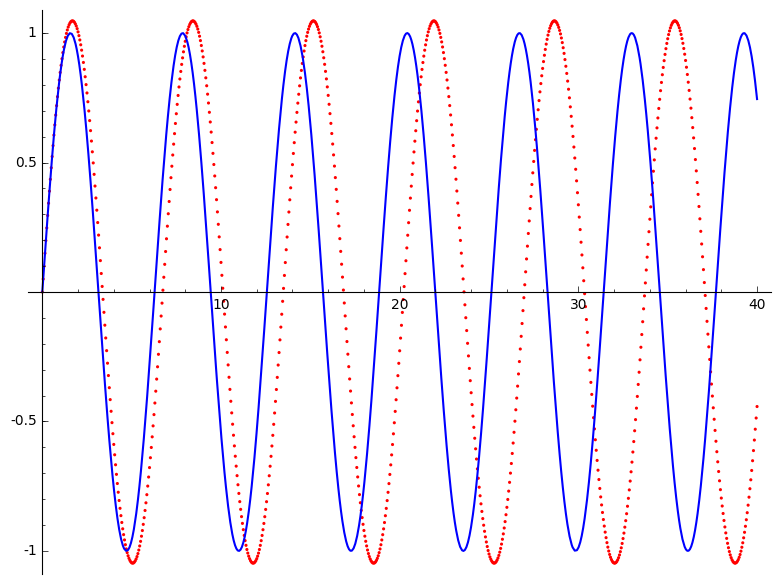
\includegraphics[width=0.65\textwidth]{images/fastTheta1.png}
			\caption{Solutions to the ODE when $\theta(0)=0$, and $\theta'(0)=1$}
			\label{fastTheta1}
		\end{figure}
		\end{proof}
		% subsection part_f (end)

		\subsection*{Part (g)}
		Repeat the previous part for $\theta'(0) = 2$. 
		There is a big difference in the graphs this time. 
		Explain physically what is happening with the true pendulum.

		\begin{proof}[Solution]
		Observe Figure \ref{fastTheta2} for the graph when $\theta'_{0} = 2$.
		In this case, it helps to recall the solution when $\theta_{0}=3.1415$ and $\theta'_{0} = 0$.
		There, we saw the pendulum hang at its maximum angle (and maximum height) for quite awhile before falling again.
		The difference here, is that instead of starting from a high location, it is being swung there by an external force, and then left to its own devices.

		\begin{figure}[b]
			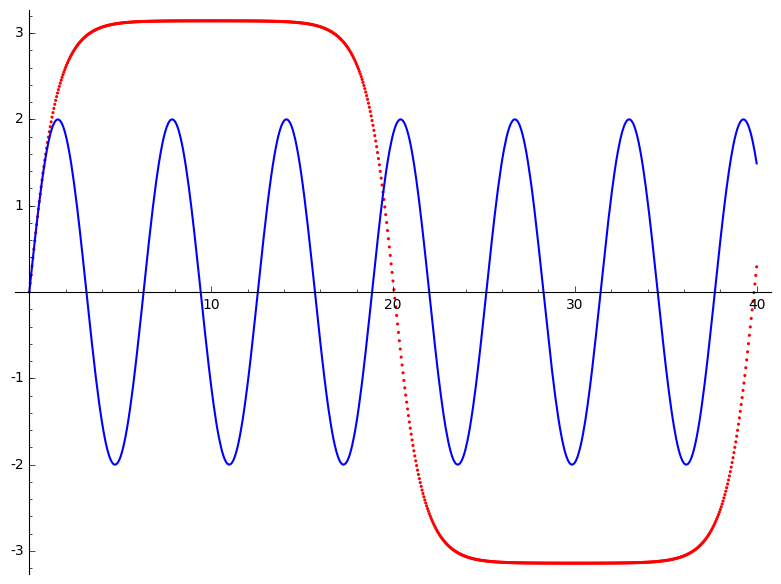
\includegraphics[width=0.65\textwidth]{images/fastTheta2.png}
			\caption{Solutions to the ODE when $\theta(0)=0$, and $\theta'(0)=2$}
			\label{fastTheta2}
		\end{figure}
		\end{proof}
		% subsection part_g (end)

		\subsection*{Part (h)}
		Now try $\theta'(0) = 2.01$. 
		The graph should be very different now! 
		Sage is not doing anything wrong, and this is the true physical solution. 
		Explain what is happening here.

		\begin{proof}[Solution]
		In Figure \ref{fastTheta3} we have the very amusing result that if the initial angular velocity is slightly greater than 2, then the pendulum swings in a circle without slowing down.

		\begin{figure}[b]
			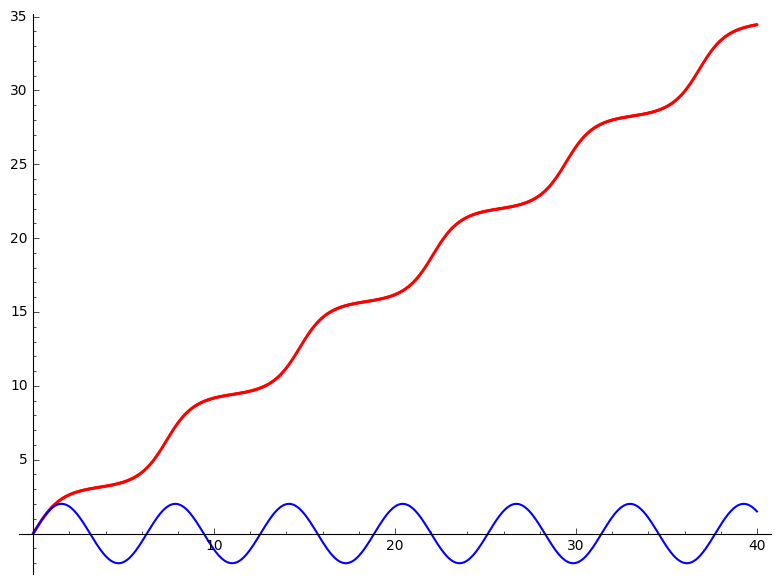
\includegraphics[width=0.65\textwidth]{images/fastTheta3.png}
			\caption{Solutions to the ODE when $\theta(0)=0$, and $\theta'(0)=2.01$}
			\label{fastTheta3}
		\end{figure}
		\end{proof}
		% subsection part_h (end)
	% section exercise_3 (end)
\end{document}